\section{Additional Analysis}

\subsection{Detailed Results}
%% Class F1 scores
Figure~\ref{fig:class_f1_sato} shows the F1 score of \name{} and Sato for each class on the VizNet (Full) and VizNet (Multi-column only) datasets. 
%
The improvements against Sato on the two variants of the VizNet datasets indicate that \name{} robustly and consistently performs better than Sato, especially for single-column tables, where Sato cannot benefit from the table features and CRF.
%
We found that Sato shows zero or very poor F1 values for {\tt religion}, {\tt education}, {\tt organisation}.
%
\hl{The labeled columns in the training data in the 1st fold of the VizNet (Full) are only 24, 22, and 14, respectively. Sato should suffer from the lack of training examples for those column types, and probably the skewed column type distribution as well. We show that \name{} robustly performs well on such column types.}


Table~\ref{tab:tur_class_f1} shows the performance of \name{} and \namest{} on the WikiTable dataset for 6 column types/column relations.
%
We confirm that \name{} tends to perform better for the column types/relations that are less clearly distinguishable (e.g., artist vs. writer, place-of-birth vs. place-lived.)


\begin{figure*}[t]
         \centering
         \begin{subfigure}[b]{0.95\textwidth}
             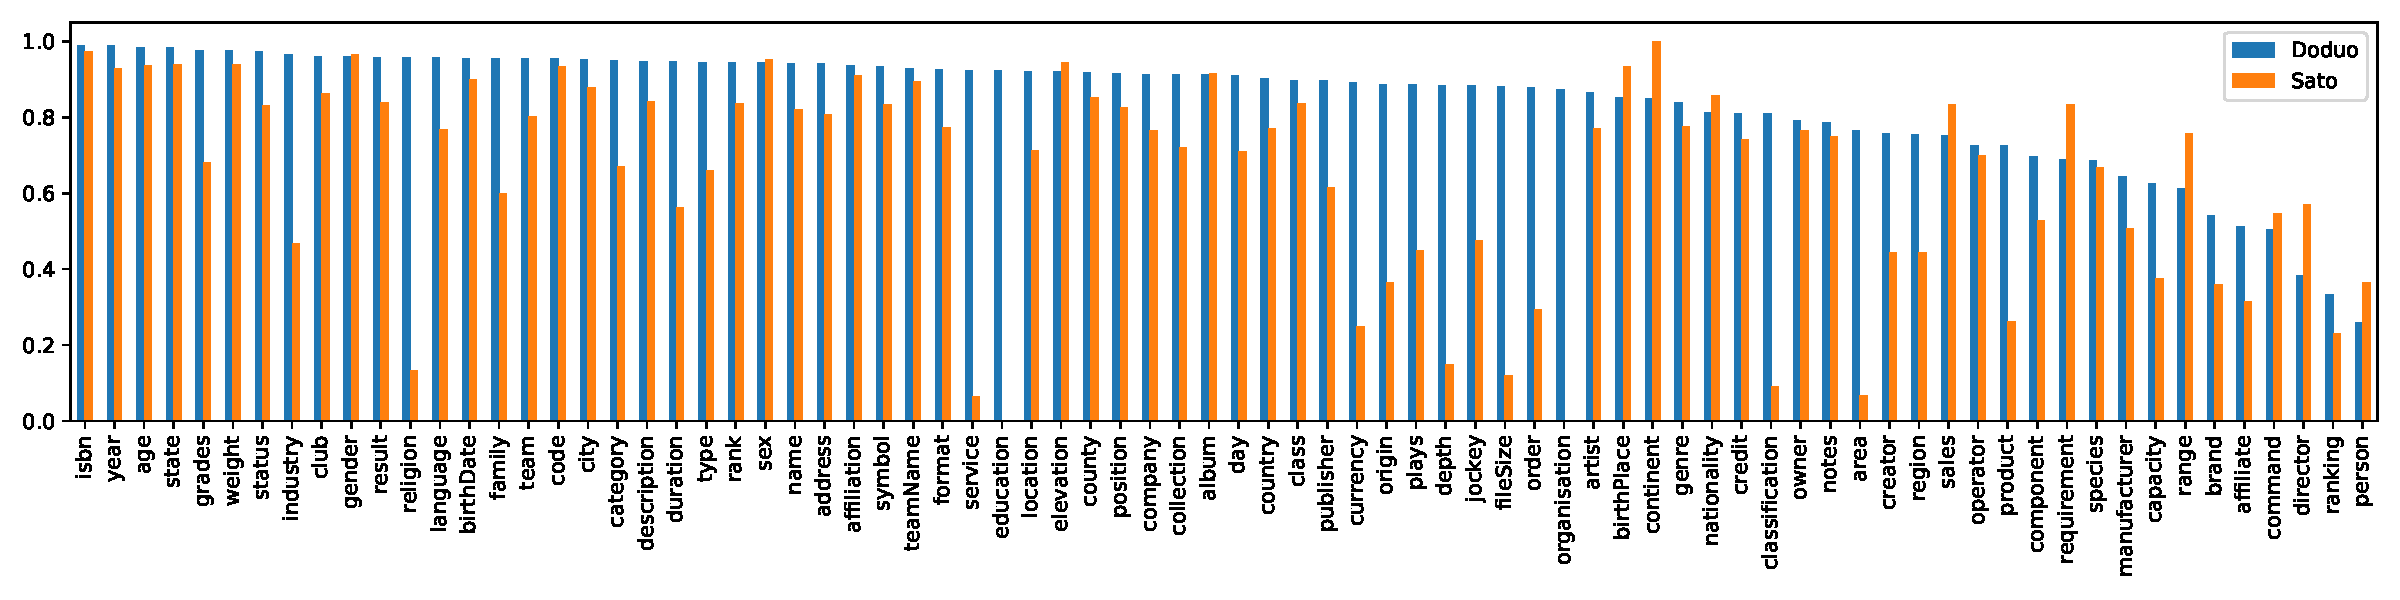
\includegraphics[width=\textwidth]{fig/viznet_doduo_sato_class_f1_full.pdf}
         \end{subfigure}
         \begin{subfigure}[b]{0.95\textwidth}
             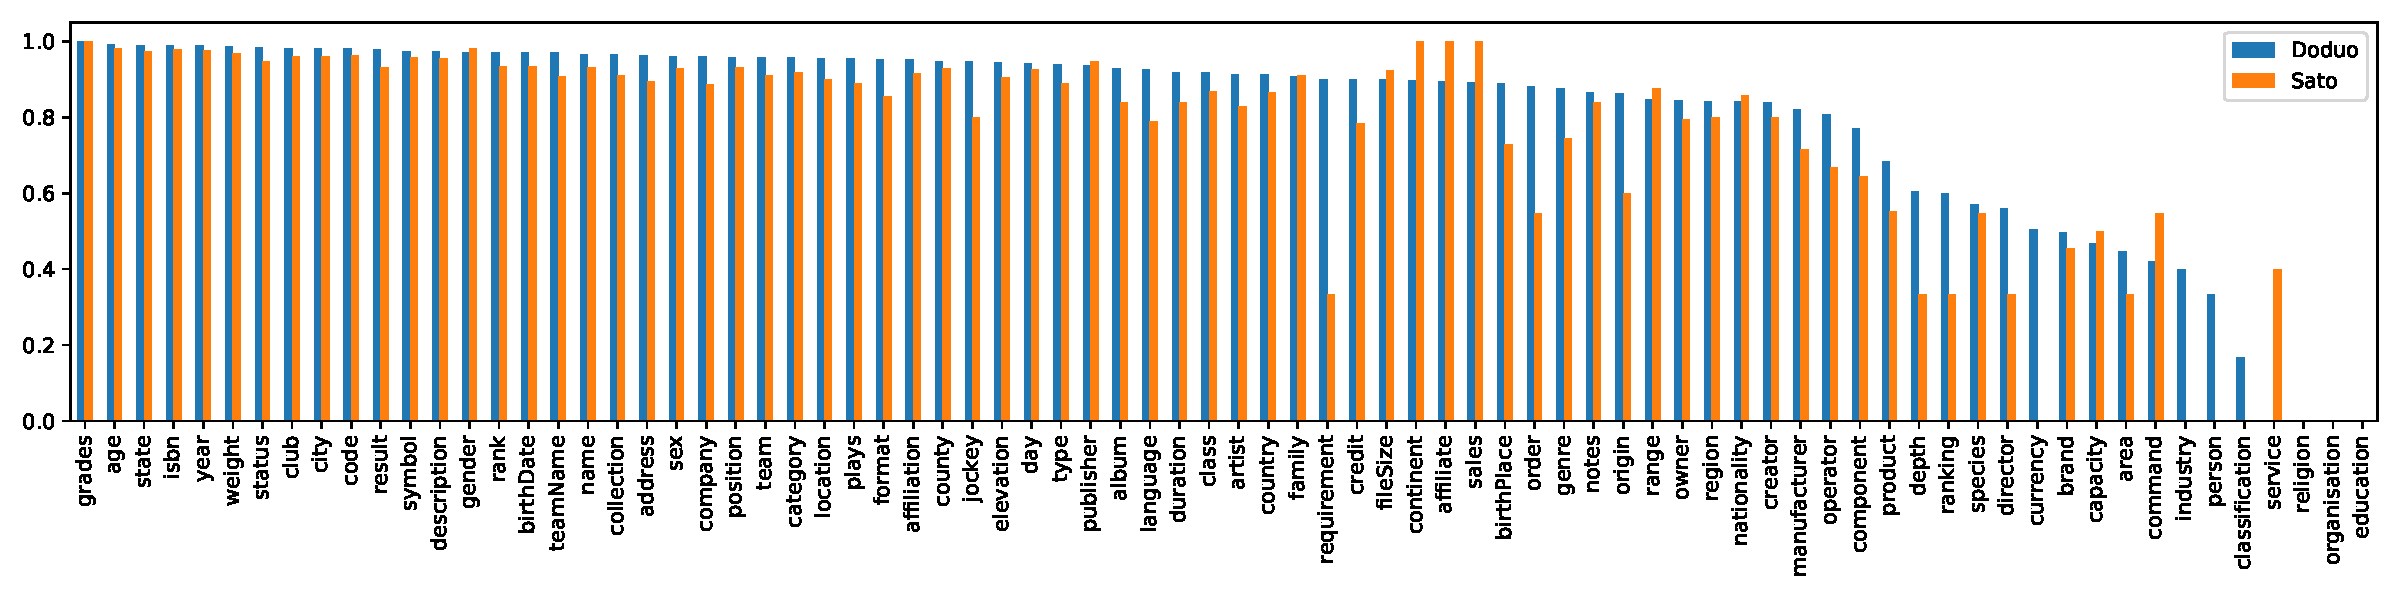
\includegraphics[width=\textwidth]{fig/viznet_doduo_sato_class_f1_multicol.pdf}
         \end{subfigure}
         \caption{Class F1 values by \name{} and Sato on the VizNet dataset (Above: Full set; Below: Multi-column only.)}\label{fig:class_f1_sato}
\end{figure*}


\begin{table*}[t]
\caption{Further analysis on column type prediction (left) and on column relation prediction (right.)}\label{tab:tur_class_f1}
\begin{subfigure}[b]{0.49\textwidth}
    \centering
    %\footnotesize
    \small
    \begin{tabular}{p{5.1cm}|c|c}\hline
    Column type & \name{} (F1) & \namest{} (F1) \\\hline\hline
    {\tt music.artist}                          &   {\bf 84.03}  &   81.87 \\
    {\tt music.genre}                           &   {\bf 93.33}  &   87.50 \\
    {\tt music.writer}                          &   {\bf 75.00}  &   40.00 \\ 
    {\tt american\_football.football\_coach}      &  {\bf 70.59}  &   66.67 \\
    {\tt american\_football.football\_conference} &  {\bf 44.44}  &   36.36 \\
    {\tt american\_football.football\_team}       &  {\bf 86.67}  &   86.36 \\\hline
    \end{tabular}
\end{subfigure}
\begin{subfigure}[b]{0.49\textwidth}
    \centering
    %footnotesize
    \small
    \begin{tabular}{p{4.1cm}|c|c}\hline
    Column relation & \name{} (F1) & \namest{} (F1) \\\hline\hline
    {\tt film.film.production\_companies}                          & {\bf 80.95}  & 74.29 \\
    {\tt film.film.produced\_by}                                   & {\bf 43.90}  & 38.89	\\
    {\tt film.film.story\_by}                                      & {\bf 100.00} & 90.91	\\
    {\tt people.person.place\_of\_birth}                           & {\bf 92.00}  & 90.79	\\
    {\tt people.person.place\_lived} & {\bf 85.98}  & 77.67	 \\
    {\tt people.person.nationality}                                & {\bf 100.00} & 98.80 \\\hline
    \end{tabular}
\end{subfigure}
\end{table*}


\subsection{Input Token Length}

%% VizNet
For the VizNet dataset, we tested \name{} and \namesc{} with different maximum token numbers per column. 
%
Table~\ref{tab:sato_maxtoken} shows the similar trends as the results on the WikiTable dataset. \name{} with 8 max tokens per column with \name{} outperforms the state-of-the-art method (i.e., Sato) on the task.
%
As we observe significant differences between the multi-column model (\name) and the single-column model (\namesc), we consider it is mainly because the Transformer blocks (i.e., self-attention mechanisms) capture the inter-column table context successfully. 


\begin{table}[t]
\centering
\caption{Comparisons with different input token size on the VizNet (Full) dataset.}\label{tab:sato_maxtoken}
\begin{tabular}{c|c|cc}\hline
 Method & MaxToken/col & Macro F1 & Micro F1 \\\hline\hline
\name      & 8 & 81.0 & 92.5 \\
           & 16 & {\bf 83.6} & 93.6 \\
           & 32 & 83.4 & {\bf 94.2} \\\hline
\namesc    & 8 & 72.7 & 87.2 \\
           & 16 & 76.1 & 89.1 \\
           & 32 & 77.4 & 90.2 \\\hline
\end{tabular}
\end{table}




\subsection{Learning Efficiency}

\subsection{\hl{Inter-column Dependency}}\label{subsec:attention}
%% Overview
A strength of the Transformer architecture is stacked Transformer blocks that calculate highly contextual information through the self-attention mechanism.
%
As described in Section~\ref{sec:model}, \name{} uses the {\tt [CLS]} dummy symbols to explicitly obtain contextualized column representations. The representations not only take into account table context but also explicitly incorporate the inter-column dependency. That is, as we showed in Figure~\ref{fig:examples}, predictions for some columns should be relevant and useful for other columns in the table.
%
To the best of our knowledge, none of the existing work that applies pre-trained LMs to tables has conducted this type of analysis for better understanding how the Transformer-based model captures the semantics of tables.


%%
Thus, we conduct attention analysis to further understand how the attention mechanisms of \name{} (i.e., the pre-trained LM) captures the inter-column dependency and the semantic similarity between them.
%
Following the literature of attention analysis in NLP~\cite{Clark:2019:WhatDoesBERTLookAt,tenney-etal-2019-bert-rediscovers,Rogers:2020:TACL:BERTology}, we look into attention weights for the analysis.
%
It is known that in pre-trained Transformer-based LMs, 
%
the deep layer focuses on semantic similarity between tokens~\cite{Clark:2019:WhatDoesBERTLookAt,tenney-etal-2019-bert-rediscovers}.
%
Therefore, to investigate the high-level (semantic) similarity between columns, we looked into the attention weights of the last Transformer block. 
%

%% Details
We used the VizNet dataset (Multi-column only) for the analysis.
%
Specifically, we focus on attention weights between {\tt [CLS]} tokens (i.e., column representations.) 
%
Since Transformer-based LMs usually have multiple attention heads (e.g., 12 heads in the BERT Base model,) we aggregate attention weights of all attention heads. As a result, we obtain an $S \times S$ matrix, where $S$ denotes the input sequence length.
%
We disregard aggregated attention weights other than those for {\tt [CLS]} tokens.
%
\hl{After masking out any attention weights other than {\tt [CLS]} tokens, we averaged the matrices obtained from all tables in the dataset so that we can create a single $|\mathcal{C}_{\rm type}| \times |\mathcal{C}_{\rm type}|$ matrix that represents the dependency between column types. This gives us aggregated information about the dependency between column types.}


Each element ($i$, $j$) in the final matrix represents how much the column type $i$ relies on the other column type $j$ for its contextualized representation.
%
Note that the \hl{dependency} of column type $i$ (or $j$) for column type $j$ (or $i$) can be different, and thus the matrix is not symmetric. \hl{For example, {\tt age} highly relies on the type {\tt origin}, whereas the opposite direction has negative attention weight showing a low degree of dependency.}
%
To eliminate the influence of the co-occurrence of column types, we counted the co-occurrence of column types in the same table and \hl{normalized the matrix to make the reference point to be zero for more straightforward interpretation.
%
As a result, the final matrix consists of relative importance scores, and higher/lower values mean more/less influence from the column type.}
%


\hl{Figure~\ref{fig:attention} depicts the final matrix in heatmap visualization. Higher values (colored in red) indicate stronger dependency of column types (in $y$-axis) against other column types (in $x$-axis). For example, {\tt gender} ({\tt age}) has a higher value against {\tt country} ({\tt origin}.) We can interpret that majority of information, which composes the contextualized column representations for {\tt gender} columns, is derived from {\tt origin.} On the other hand, the {\tt gender} column seems not to be important for the {\tt origin} column.}
%
The results confirm that \name{} learns the inter-column dependency through the self-attention mechanism and the learned semantic similarity values between different pairs of column types have different weights, which the co-occurrence cannot simply explain.


\begin{figure}[t]
    \centering
    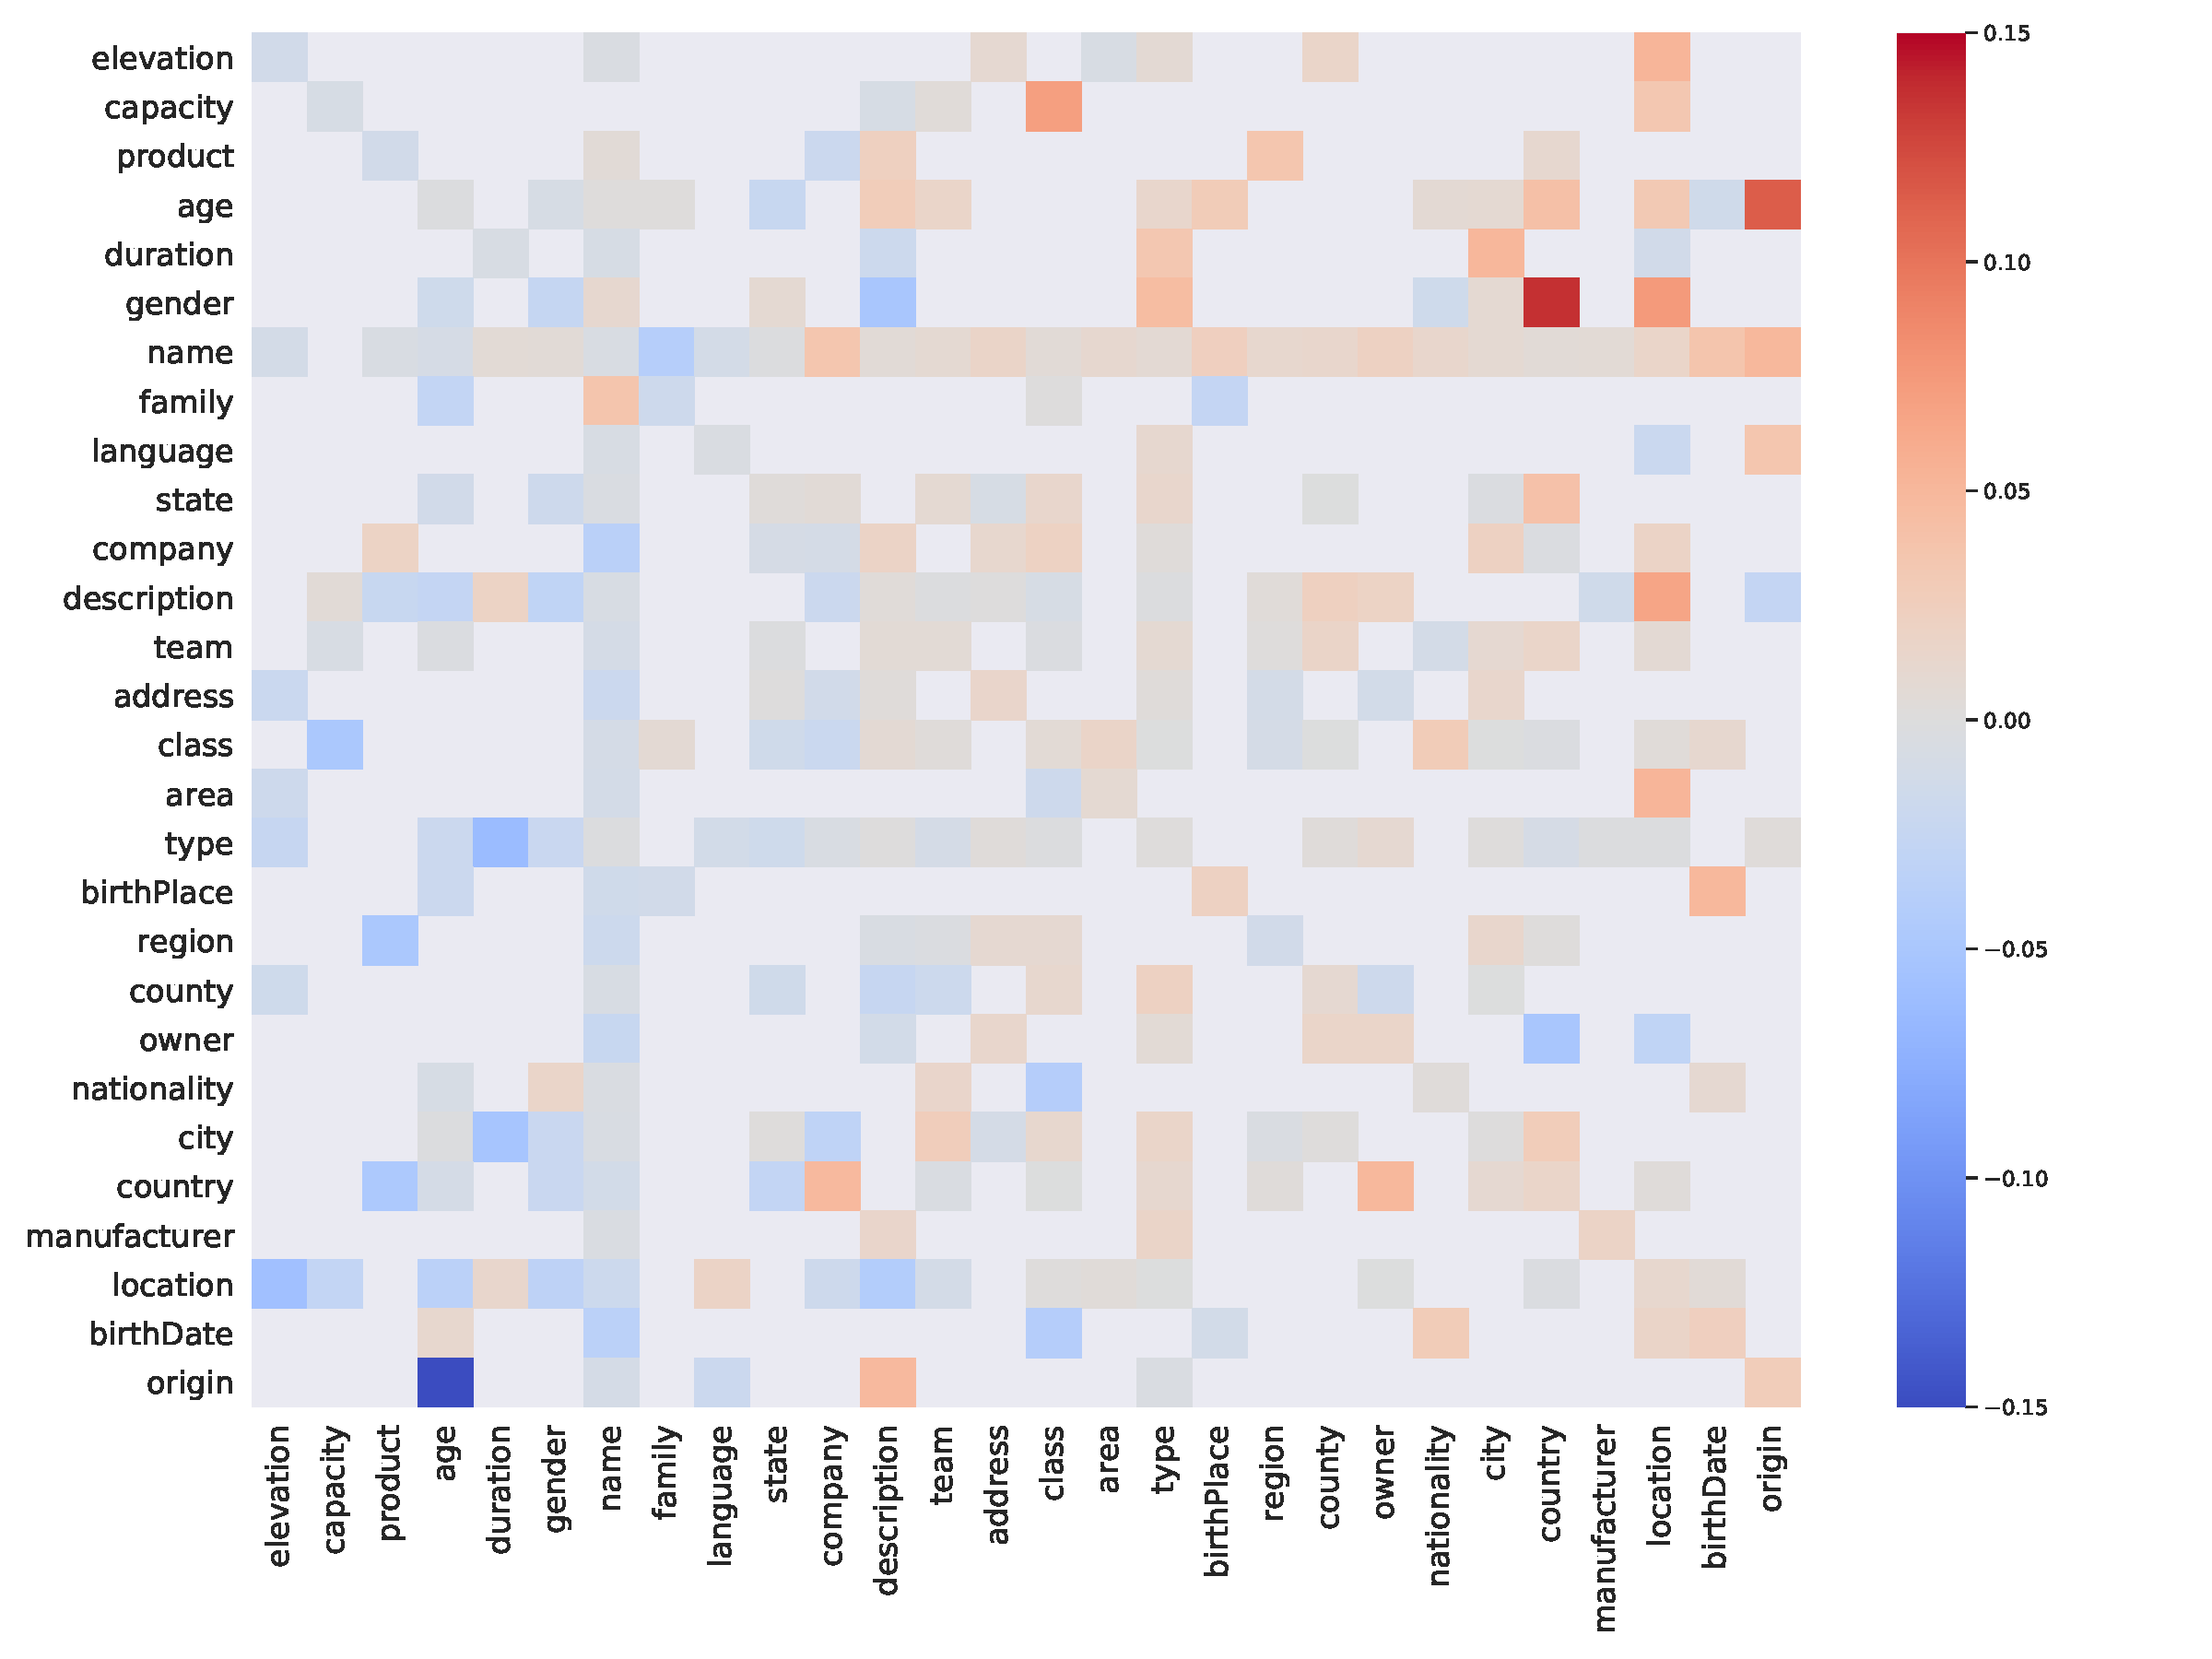
\includegraphics[width=0.50\textwidth]{fig/att_cooc_msato_cv0_mcol_doduo_filtered.pdf}
    \caption{Inter-column dependency based on attention analysis on the VizNet dataset. A higher value (red) indicates that the column type ($y$-axis) ``relies on'' the other column type ($x$-axis) for prediction. Each row denotes the degree of ``dependence'' against each column. For example, {\tt age} in $y$-axis has a high attention weight against {\tt origin} in $x$-axis, indicating that predicting {\tt age} relies on signals from the {\tt origin} column.}
    \label{fig:attention}
    \vspace{-0.5cm}
\end{figure}


\subsection{\hl{Language Model Probing}}\label{subsec:lm_probing}
% 
Recent applications of pre-trained LMs to data management tasks including entity matching~\cite{Brunner:2020:EDBT:BERT4EM,Li:2020:Ditto} and column annotation tasks~\cite{Deng:2020:TURL,Wang:2021:TCN} have shown great success by improving previous SoTA performance by a large margin.
%
However, little is known about how well pre-trained LMs {\em inherently} know about the problem in the first place. 
%
Pre-trained LMs are trained on large-scale textual corpora, and the pre-training process helps the pre-trained LM to memorize and generalize the knowledge stored in the pre-training corpus. 


% why we did this analysis
There is a line of recent work that aims to investigate how well pre-trained LMs know about factual knowledge~\cite{Petroni:2019:LAMA,Jiang:2020:HowCanWeKnowLM,Roberts:2020:HowMuchKnowledge}. The studies have shown that pre-trained LMs store a significant amount of factual knowledge through pre-training on large-scale corpora.
%
Therefore, we hypothesized that \name's performance was partly boosted by the knowledge obtained from the pre-training corpus that might store knowledge relevant to the task.
%
To verify the hypothesis, we evaluated if the BERT model, which we used as the base model for the experiments, stored relevant knowledge for the column annotation problem.

In the analysis, following the line of work~\cite{Petroni:2019:LAMA,Jiang:2020:HowCanWeKnowLM,Roberts:2020:HowMuchKnowledge}, we use the template-based approach to test if a pre-trained LM knows the factual knowledge. 
%
Specifically, we use a template that has a blank field for the column type like below:
%
\begin{center}
    Judy Morris is \_\_\_\_\_.
\end{center}
%
In this example, ``director'' should be a better fit than other column types (e.g., ``actor'', ``player'', etc.)

%% 
In this way, we conclude that the model knows the fact if the model judges the template with the true column type (e.g., ``director'') {\em more likely} than other sentences that use different column types (e.g., ``actor'', ``player'', etc.).
%
To evaluate the likelihood of a sequence after filling the blank in the template, we use the {\em perplexity} score of a sequence using the pre-trained LM.
%
Perplexity is used to measure how well the LM can predict each token from the context (i.e., the other tokens in the sequence\footnote{It would be the next token from the previous tokens if the model were an autoregressive model that only considers backward dependency in each step (e.g., GPT-2.) Since BERT has bi-directional connections between any tokens in the input sequence, the perplexity should take into account any other tokens in the input sequence to evaluate the likelihood of the target token.}) and is calculated by the average likelihood of a sequence. It is a common metric to evaluate how ``natural'' the text is from the LM perspective.
%
%
The perplexity of a sequence of tokens $X = (x_1, x_2, \dots, x_t)$ is defined by:
\begin{equation}
    PPL(X) = \exp \left\{- \frac{1}{t}\sum_i^t \log p_\theta(x_i | x_{\setminus i}) \right\},
\end{equation}
%
%
where $p_\theta(x_i | x_{\setminus i})$ denotes the probability of an LM $\theta$ (e.g., BERT) predicting a target token $x_i$ given the context in $X$ with $x_i$ masked out.
\hl{With the same LM, the lower perplexity score for a sentence indicates it is easier for the LM to generate the sentence.}


%% Explain how we evaluate the score
We use the perplexity to score column types for each column value (e.g., Judy Morris) by filling each column type name in the template. Then, we can evaluate if the ground truth label (i.e., ``director'' in this case) has the best (i.e., lowest) perplexity among all candidates. For the analysis, we use the vanilla BERT ({\tt bert-base-uncased}) model, which is the same base model used for \name{} in the experiments. 
%
We use the average rank and the normalized PPL (= PPL / Avg. PPL, where Avg. PPL denotes the average perplexity of all column types for evaluation.) 
%
Since perplexity values for sequences with different lengths are not directly comparable, we selected column types that are tokenized into a single token by the BERT tokenizer\footnote{Technically, column type names in the WikiTable contain hierarchical information, which is represented by URI. We used the leaf node as the column type name.}. As a result, 80 (out of 255) and 75 (out of 78) column types were selected for the WikiTable and VizNet datasets for the analysis, respectively.


\begin{table*}[t]
\caption{Language model probing results on the WikiTable dataset (Left: column type prediction. Right: Column relation prediction.) The average rank becomes $1$ if the language model always judges the column type (column relation) as the most ``natural'' choice among 80 (34) candidates for the target column value (the target column value pair.) We consider the language model has more {\em prior knowledge} about the column types (column relations) in Top-5 than those in Bottom-5.
}\label{tab:lm_probing_turl}
\begin{subfigure}[b]{0.49\textwidth}
\small
    \centering
    \begin{tabular}{c|c|cc}\hline
& Column type & Avg. rank ($\downarrow$) & PPL / Avg.PPL ($\downarrow$) \\\hline\hline
\multirow{5}{*}{\rotatebox{90}{Top-5}}& 
government.election  &   6.74 &  0.787 \\
& geography.river      &   9.25 & 0.788 \\
& religion.religion    &  10.10 & 0.799 \\
& book.author          &  12.72 & 0.810 \\
& education.university &  15.62 & 0.829 \\\hline
\multirow{5}{*}{\rotatebox{90}{Bottom-5}}& 
royalty.monarch         &  58.24 & 1.147 \\
& astronomy.constellation &  67.47 & 1.170 \\
& law.invention           &  61.60 & 1.181 \\
& biology.organism        &  71.56 & 1.205 \\
& royalty.kingdom         &  73.37 & 1.368 \\\hline
    \end{tabular}
    \footnotesize
\end{subfigure}
\begin{subfigure}[b]{0.49\textwidth}
    \centering
    \small
    %\footnotesize
    \begin{tabular}{c|c|cc}\hline
& Column relation & Avg. rank ($\downarrow$) & PPL / Avg.PPL ($\downarrow$) \\\hline\hline
\multirow{5}{*}{\rotatebox{90}{Top-5}}&
person.place\_of\_birth                       &  3.69 &   0.946 \\
& baseball\_player.position\_s                &  5.04 &   0.961 \\
& location.nearby\_airports                  &  8.66 &    0.979 \\
& mailing\_address.citytown                  &  7.24 &    0.980 \\
& film.directed\_by                              &  8.08 &  0.984 \\\hline
\multirow{5}{*}{\rotatebox{90}{Bottom-5}}& 
award.award\_nominee &  16.53 &         1.019 \\
& tv\_program.country\_of\_origin &  16.83 &         1.030 \\
& country.languages\_spoken       &  14.79 &         1.042 \\
& award\_honor.award\_winner &  21.40 &               1.047 \\
& event.entity\_involved           &  19.82 &         1.072 \\\hline
    \end{tabular}    
\end{subfigure}
\end{table*}



\begin{table}[t]
\small
    \centering
    \caption{Language model probing results on the VizNet dataset. We observe that the language model stores a certain amount of factual knowledge about column types listed in Top-5, compared to Bottom-5. The general trend is consistent with Table~\ref{tab:lm_probing_turl}.     
}
    \label{tab:lm_probing_sato}
    \begin{tabular}{c|c|cc}\hline
& Column type & Avg. rank ($\downarrow$) & PPL / Avg.PPL ($\downarrow$) \\\hline\hline
\multirow{5}{*}{\rotatebox{90}{Top-5}}& year         &   6.60 & 0.799 \\
& manufacturer &  20.19 & 0.810 \\
& day          &  14.21 & 0.819 \\
& state        &  16.88 & 0.825 \\
& language     &  17.23 & 0.840 \\\hline
\multirow{5}{*}{\rotatebox{90}{Bottom-5}}&
organisation &  61.83 & 1.146 \\
& nationality  &  65.81 & 1.218 \\
& creator      &  57.39 & 1.232 \\
& affiliation  &  63.85 & 1.239 \\
& birthPlace   &  72.30 & 1.334 \\\hline
    \end{tabular}
\end{table}



%% Relation prediction
We can use the same framework for the column relation prediction task as well. In this case, we consider a different template that has a blank field for the column relation. For example,
%
\begin{center}
    Derrick Henry \_\_\_\_\_ Yulee, Florida.
\end{center}
%
In this example, the likelihood of a sentence with ``was born in'' ({\tt place\_of\_birth}) should be judged higher than that with ``was died in'' ({\tt place\_of\_death}), which requires factual knowledge about the person. Since the column relation types are not written in plain language, we manually converted column relation type names so that they better fit in the template ({\tt entity 1}, {\tt relation}, {\tt entity 2}). Examples of converted column relation names are ({\tt place\_of\_birth}, ``was born in''), 
({\tt directed\_by}, ``is directed by''). We filtered 34 (out of 121) column relation types to make sure the converted relation type names have the exact same number of tokens. 


%% Training a model from scratch
As a more direct way to test the hypothesis, we also evaluated a variant of \name{} that randomly initialized model parameters instead of using the pre-trained parameters of BERT. In this way, we can test the performance when the model with the identical architecture is trained from scratch only using training data of the target task. The model did not show meaningful performance (i.e., \hl{approximately zero F1 value}.)
%
We consider this is mainly because the model is too large to be trained on only the training data (i.e., without pre-training.) Thus, we decided to use the ``language model probing'' method to test the hypothesis.


\smallskip
\noindent
{\bf Results.} Table \ref{tab:lm_probing_turl} shows the results on the WikiTable dataset. We observe that some column types (e.g., goverment.election, geography.river) show lower average rank and PPL / Avg. PPL (i.e., the BERT model knows about the facts), whereas some column types (e.g., biology.organism, royalty.kingdom) show poor performance on the language probing analysis.
%
For example, the ``government.election'' column type is ranked at 6.74 on average and shows a smaller PPL than the average PPL. That means values in the columns that have the ``government.election'' ground-truth labels are considered ``more natural'' to appear with the term ``election''\footnote{Again, we used the leaf node of each column type as the term for the template.} than other column type names by the pre-trained LM (i.e., BERT.)
%
As we used 80 column types for the analysis, the ``royalty.kingdom'' column type is almost always ranked at the bottom by the LM. The poor performance could be attributed to the lower frequency of the term ``kingdom'' than other terms in the pre-training corpus.


%% Relation
For the column relations on the WikiTable dataset, the results in Table~\ref{tab:lm_probing_turl} (Right) indicate that the LM knows about factual knowledge of persons as the probing performance for relations such as {\tt place\_of\_birth} and {\tt position} is higher.
%
Compared to the probing results for the column types, the results show less significant differences between top-5 and bottom column relations. This is mainly because the template has three blank fields for two entities and one relation, which has a higher chance to create an unnatural sentence for the LM than that for column types.


%% Column type
The probing analysis on the VizNet dataset shows the same trend as in the WikiTable dataset. In Figure~\ref{fig:class_f1_sato}, we confirm that \name{} has better performance than Sato for all the top-5 column types. Meanwhile, {\tt birthPlace} and {\tt nationality}, which are in the bottom-5 column types for the language model probing analysis, are among the few column types where \name{} underperforms Sato. The results support that \name{} may not benefit from relevant factual knowledge stored in the pre-trained LM for the column type.


%%
Note that the BERT model used for the analysis is {\em not fine-tuned} on the WikiTable/VizNet dataset, but the vanilla BERT model. Thus, the language model probing analysis shows the inherent ability of the BERT model, and we confirm that the pre-trained LM does store factual knowledge that is useful for the column annotation problem. 
%
This especially explains the significant improvements over the previous SoTA method that does not use pre-trained LM (i.e., Sato), as shown in Figure~\ref{fig:class_f1_sato}.


\section{Limitations and Future Work}\label{sec:discussion}
We have discussed why \name{} performs well for the column annotation problem through the series of analysis. In this section, we summarize the limitations of \name{} and our findings in the paper to discuss open questions for future work.

%% Table value only
\noindent
{\bf Table values only vs. with meta information.}
First, \name{} takes table value only. In most cases, we believe this assumption makes the framework more flexible to be practical.
%
For example, spreadsheets and data frames, which are common data format choices for data analysis, do not have table captions and often lack meaningful table headers.
%
Nevertheless, we acknowledge that, in some cases, meta information plays an important role to complementing table values to compose the table semantics.
%
As recent work~\cite{Deng:2020:TURL,Wang:2021:TCN} has shown the effectiveness of meta information for the table tasks, understanding when meta information becomes essential for the task is still an open question.


%% Assumption: a table contains multiple tables
\noindent
{\bf Single-table model vs. multi-table model.}
Second, \name{} assumes the input table to be {\em self-contained.} That means columns that are necessary to compose table context should be stored in the same table.
%
Web Tables generally follow the assumption, and \name{} shows the strong performance on the WikiTable and VizNet datasets.
%
However, \name{} was not tested on relational tables, where chunks of information can be split into multiple tables after database normalization.
%
In such a scenario, we need to consider inter-table relations and information to incorporate key signals outside the target table.
%
In fact, contemporaneous work~\cite{Wang:2021:TCN} has developed a framework that incorporates signals from external tables for better column annotation performance.
%
Thus, we consider joint modeling of multiple tables should be a future direction.


%% Dirty data, although it is known that pre-trained models are known to be robust for dirty data. 
\noindent
{\bf Clean data vs. dirty data.}
Third, our framework assumes that table values are ``correct and clean'', which may not always be true in real-world settings.
%
The input table value should be of the high-quality, especially when we limit the max input token size for better efficiency.
%
Recent studies that applied pre-trained LMs to tables~\cite{Li:2020:Ditto,Li:2021:JDIQ:DeepEntityMatching} have shown that the pre-trained LM-based approach achieves robust improvements even on ``dirty'' datasets, where some table values are missing or misplaced.
%
Following the error detection/correction research~\cite{Mahdavi:2019:Raha,Mahdavi:2020:Baran}, which has been studied independently, implementing functionality that alleviates the influence from the incorrect table values is part of the future work.


%% More tasks, and task similarity.
\noindent
{\bf Multi-task learning with more tasks.}
Lastly and most importantly, there are many open questions in applying multi-task learning to data management tasks. Although we have shown that multi-task learning is useful for the column annotation task, it is not yet very clear what types of relevant tasks are useful for the target task.
%
A line of work in Machine Learning has studies on the task similarity and the transferability of the model~\cite{Taskonomy2018}.
%
Therefore, it is also important for us to understand the relationship between task similarity and benefits of the multi-task learning framework.
%
We acknowledge that our study is still preliminary with respect to this point. However, we believe that our study established the first step in this research topic toward a wider scope of multi-task learning applicability to other data management tasks.


